\documentclass[10pt]{article}
\usepackage[letterpaper,left=1.15in,right=1.15in,top=1in,bottom=1in]{geometry}
\usepackage{newtxtext,newtxmath}
\usepackage{booktabs}
\usepackage{graphicx}
\usepackage{amsmath}
\usepackage[hidelinks]{hyperref}
\usepackage{caption}
\graphicspath{{figures/}{../artifacts/analysis/}}
\captionsetup{font=small,labelfont=bf}
\setlength{\parskip}{2pt}

\title{\vspace{-1.4em}\bf Price Images as a Representation:\\ Replicating and Stress-Testing a CNN for 20-Day Return Prediction}
\author{PENG You \quad MSDM5054 Final Project}
\date{}

\begin{document}
\maketitle
\vspace{-1.6em}

\begin{abstract}
\noindent
Jiang, Kelly, and Xiu (2023) encode past prices as images and report that a convolutional network reads predictive structure out of them. We replicate their 20-day specification on the course panel (1993--2019) and ask three questions that the original performance table leaves open. First, does the image representation carry out-of-sample information beyond models that see exactly the same pixels, namely a linear model and an MLP? Second, does the probability ranking survive as a portfolio once the annualisation is done correctly, trading costs are charged, and the sample is split by period? Third, is the dependence the network learns a stable price shape or a property of particular historical stretches? We train every model on three seeds and report the variation. On 1.49 million out-of-sample rows the CNN reaches an AUC of $0.530\pm0.004$ against $0.527\pm0.001$ for the MLP and $0.525\pm0.001$ for the linear model. The top-decile long--short portfolio earns seed-average Sharpe ratios of $1.70\pm0.35$ for the CNN, $1.94\pm0.18$ for the linear model, and $1.60\pm0.12$ for the MLP; averaging the three seeds' probabilities gives 1.88, 1.99, and 1.65, and net of 10 basis points 1.51, 1.46, and 1.29. The classification gain is small and inside seed variation, and it does not translate into a reliable portfolio advantage. The economic separation is real for all three models but concentrated before 2013. A column-occlusion test shows that predictions depend most on the three most recent columns of the image, and that Grad-CAM highlights columns that matter more than random columns but less than recency itself. We read the evidence as a representation that is informative, locally faithful, and strongly non-stationary, rather than as evidence of a transferable price shape.
\end{abstract}

\section{Introduction}

The empirical asset-pricing literature has long treated predictors as hand-built features. Jiang, Kelly, and Xiu (2023) instead render a window of past prices as a small image and let a convolutional network learn the mapping from image to future return. Their claim is that the image is not a convenience but a representation: local convolutions and weight sharing match the translation structure of price charts, so the network can pick up shapes that linear models cannot express.

Replication on a new sample can confirm a number or it can interrogate the reason the number appears. We take the second route and organise the study around three questions.

\textbf{Q1 (representation and inductive bias).} Given identical image inputs, does a convolutional architecture extract out-of-sample information that a linear model and an MLP do not? The three models differ only in how they combine the same 3{,}840 pixels, so a gap isolates the contribution of local connectivity and weight sharing.

\textbf{Q2 (economic validity and stability).} Does the probability ranking produce a decile portfolio separation that survives the correct annualisation, transaction costs, and a split into early and late periods? A ranking can be statistically informative and still fail to be economically meaningful, and a strategy that works only in one stretch of history is a different object from one that works throughout.

\textbf{Q3 (shape or period artefact).} Is the dependence learned by the network a stable price shape, or a statistical regularity of particular years? We approach this with architecture ablations, Grad-CAM, and a quantitative occlusion test that removes the columns the network attends to and measures how much the prediction moves.

Our answers are precise but less flattering than a leaderboard. Averaged over three seeds the CNN is the best of the three models on AUC and average precision, by 0.0025 over the MLP and 0.0049 over the linear model, against its own seed standard deviation of 0.0038. Its portfolio Sharpe ratio averages 1.70 with a seed standard deviation of 0.35; the linear model averages 1.94 with 0.18. The ranking separation is larger in relative terms than the classification gap, which is what a tail-based strategy needs, yet it is concentrated before 2013 and shrinks afterwards for every model. The occlusion test locates the network's dependence at the right edge of the image, the most recent trading days, which is consistent with a short-horizon momentum signal rather than with a reusable chart pattern.

\section{Data and protocol}

\textbf{Data.} The course provides 27 yearly pairs of image and label files for the 20-day horizon, 1993--2019. Each image is $64\times60$: 60 columns of trading days, 64 rows covering open, high, low, close, moving averages, and volume bars. Labels are 1 for a positive 20-day forward return, 0 otherwise, and 2 for missing. After dropping missing labels we keep 2{,}181{,}781 samples with a positive rate of 50.6\%.

\textbf{Split.} Following the course protocol, 1993--1999 is the development sample, split 70/30 at random into training (482{,}925) and validation (206{,}969) sets; 2000--2019 is the out-of-sample test set (1{,}491{,}887 rows, 240 monthly cross-sections). The test set is never used for model selection. This differs from the paper, which uses 1993--2000 for development and 2001--2019 for testing; we note the difference wherever it could matter.

\textbf{Normalisation.} Pixel mean and standard deviation are computed on the training split only ($\mu=0.1069$, $\sigma=0.3090$) and applied unchanged to validation and test. Computing them on the full sample would leak test information into every model, and it is the kind of detail that quietly inflates replication results.

\textbf{Models.} All three models consume the same normalised image. Logistic regression is a single linear layer over the flattened image. The MLP is one hidden layer of 128 units with ReLU and dropout 0.25. The CNN follows the paper's 20-day configuration: three convolutional blocks with $5\times3$ kernels, $2\times1$ max pooling, vertical stride 3 and vertical dilation 2 in the first block, 64/128/256 filters, batch normalisation before a LeakyReLU with slope 0.01, 50\% dropout before the classifier, and Xavier initialisation; it has 708{,}866 parameters. All models are trained with cross-entropy, Adam at $10^{-5}$, batch size 128, and early stopping after two epochs without validation improvement, as in the paper. We report the checkpoint with the lowest validation loss.

\textbf{Runs.} We train each model three times, with seeds 7, 17, and 27, on the full sample, using one V100 GPU with mixed precision. The CNN runs between 5 and 16 epochs, the MLP 8 to 9, and the linear model 18 to 22; early stopping selects a checkpoint in each case. An earlier single run of the same protocol on a hosted Kaggle GPU serves as an independent repeat and reproduces the same order of magnitude on every metric.

\textbf{Portfolio construction.} For each of the 240 test dates we rank stocks by predicted probability, go long the top decile and short the bottom decile with equal weights, and hold for the 20 trading days until the next cross-section. The portfolio return is the difference between the mean returns of the two legs. Because the cross-sections are monthly, the Sharpe ratio is annualised with 12 periods per year, $\text{SR}=\bar r/\hat\sigma\sqrt{12}$; annualising a 240-month series with the daily convention of 252 overstates the ratio by $\sqrt{21}\approx4.6$. The weights on the two legs sum to $+1$ and $-1$, so the book carries gross exposure 2. Turnover is $\tau_t=\tfrac12\sum_i|w_{i,t}-w_{i,t-1}|$, and a one-way cost $c$ in basis points is charged as $2c\,\tau_t$, because each unit of $\tau$ corresponds to two units of traded notional in a two-leg book. We also report the top/bottom 20\% sensitivity.

\section{Question 1: does the image representation add information?}

Table~\ref{tab:classification} reports out-of-sample classification metrics averaged over the three seeds. The ordering on AUC and average precision is CNN, then MLP, then logistic, but the gaps are small. The CNN gains 0.0049 of AUC over the linear model and 0.0025 over the MLP, with accuracy rising from 51.67\% to 51.74\% for the MLP and falling to 51.47\% for the CNN, which trades recall for precision at the 0.5 threshold.

\begin{table}[t]
\centering
\small
\caption{Out-of-sample classification, 2000--2019 (1{,}491{,}887 rows), mean $\pm$ standard deviation over seeds 7, 17, and 27. Threshold 0.5.}
\label{tab:classification}
\begin{tabular}{lccc}
\toprule
Model & Accuracy & ROC-AUC & Average precision \\
\midrule
Logistic & $0.5167\pm0.0005$ & $0.5251\pm0.0008$ & $0.5255\pm0.0009$ \\
MLP      & $0.5174\pm0.0002$ & $0.5275\pm0.0009$ & $0.5272\pm0.0006$ \\
CNN      & $0.5147\pm0.0074$ & $0.5300\pm0.0038$ & $0.5282\pm0.0037$ \\
\bottomrule
\end{tabular}
\end{table}

The gaps have to be read against seed variation. The CNN's AUC itself moves by 0.0038 across seeds, twice the size of its lead over the MLP and about 4.7 times its lead over the linear model; the MLP and the linear model are far more stable, with seed standard deviations below 0.001. A single run, such as our first Kaggle run with AUC 0.5357, would have shown a lead of 1.1 points over the linear model; the seed average shows 0.49 points, and the best seed is not systematically the same one across metrics. The honest reading is that the convolutional prior adds a small amount of information, of the same order as the run-to-run noise that any single training run carries.

The gap is also not constant over time. Splitting the test period into three blocks (Table~\ref{tab:subperiod-auc}), the CNN AUC is 0.533 in 2000--2004, 0.539 in 2005--2012, and 0.516 in 2013--2019; the linear model moves from 0.531 to 0.512 over the same blocks. The CNN advantage is largest in the middle period, at about 0.006, and smallest at the end, at about 0.004, while the absolute level of every model falls in the last block.

\begin{table}[t]
\centering
\small
\caption{ROC-AUC by test subperiod, mean $\pm$ standard deviation over seeds 7, 17, and 27. The absolute level of every model falls in 2013--2019.}
\label{tab:subperiod-auc}
\begin{tabular}{lccc}
\toprule
Model & 2000--2004 & 2005--2012 & 2013--2019 \\
\midrule
Logistic & $0.5306\pm0.0011$ & $0.5319\pm0.0013$ & $0.5113\pm0.0012$ \\
MLP      & $0.5313\pm0.0004$ & $0.5350\pm0.0013$ & $0.5147\pm0.0013$ \\
CNN      & $0.5329\pm0.0056$ & $0.5391\pm0.0014$ & $0.5156\pm0.0051$ \\
\bottomrule
\end{tabular}
\end{table}

We therefore answer Q1 with a qualified yes. The convolutional prior adds information on this sample and the gain is reproducible in sign across seeds and metrics, but it is small, comparable to seed noise, and it does not widen over time. Whatever the network extracts, a linear map over the same pixels already captures most of it.

\section{Question 2: does the ranking become an economically meaningful portfolio?}

Table~\ref{tab:portfolio} reports the top-decile long--short portfolio. Averaged over seeds, the linear model earns the highest Sharpe ratio, 1.94, against 1.70 for the CNN and 1.60 for the MLP; the CNN's seed standard deviation of 0.35 is about twice that of the other two models, and its individual seeds range from 1.46 to 2.10. The CNN's seed-average cumulative gross return, 70.9, hides seeds that end at 17.1, 214.7, and 12.1 times; its median is 17.1, close to the linear model's 17.4. Averaging the three seeds' probabilities removes part of that variation and gives Sharpe ratios of 1.99 for the linear model, 1.88 for the CNN, and 1.65 for the MLP, with $t$-statistics of 8.90, 8.39, and 7.39, Newey--West $t$-statistics of 7.03, 7.07, and 6.12, and moving-block bootstrap 95\% intervals of $[1.61,2.44]$, $[1.50,2.75]$, and $[1.33,2.43]$. Seed-averaged cumulative gross returns over 240 months are 20.9, 70.9, and 28.7 times.

\begin{table}[t]
\centering
\small
\caption{Top/bottom-decile long--short portfolio, 240 monthly cross-sections, annualised with 12 periods. Panel A: mean $\pm$ standard deviation over seeds 7, 17, and 27. Panel B: probabilities averaged over the three seeds.}
\label{tab:portfolio}
\begin{tabular}{lccc}
\toprule
\multicolumn{4}{l}{\emph{Panel A: seed averages}} \\
Model & Sharpe & 20\% Sharpe & Net Sharpe (10 bps) \\
\midrule
Logistic & $1.94\pm0.18$ & $1.85\pm0.12$ & $1.38\pm0.17$ \\
MLP      & $1.60\pm0.12$ & $1.54\pm0.09$ & $1.21\pm0.09$ \\
CNN      & $1.70\pm0.35$ & $1.67\pm0.32$ & $1.28\pm0.43$ \\
\midrule
\multicolumn{4}{l}{\emph{Panel B: seed-averaged probabilities}} \\
Model & Mean (\%) & Vol (\%) & Sharpe \\
\midrule
Logistic & 1.32 & 7.96 & 1.99 \\
MLP      & 1.47 & 10.64 & 1.65 \\
CNN      & 1.85 & 11.83 & 1.88 \\
\bottomrule
\end{tabular}
\end{table}

Figure~\ref{fig:cumulative} shows the cumulative paths. Two features matter more than the endpoint. The three models track each other closely until about 2008 and diverge afterwards; the CNN's large cumulative return is produced by a persistent spread in 2008--2012, not by a uniform advantage, and its seed-to-seed dispersion is visible in the individual paths behind the average. Net of 10 basis points the CNN path remains the highest, at a Sharpe ratio of 1.51 against 1.46 for the linear model and 1.29 for the MLP.

\begin{figure}[t]
\centering
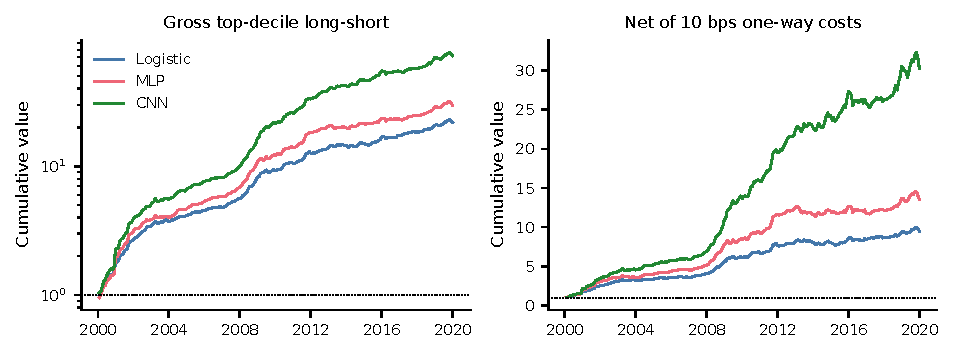
\includegraphics[width=\linewidth]{figures/cumulative.pdf}
\caption{Cumulative value of the top-decile long--short portfolio, gross (left) and net of 10 bps one-way costs (right), 2000--2019, probabilities averaged over seeds 7, 17, and 27. The y-axis is logarithmic on the left panel.}
\label{fig:cumulative}
\end{figure}

The monthly means by predicted decile (Figure~\ref{fig:deciles}) rise almost monotonically for all three models, which is the property a ranking strategy needs; the CNN's spread between the extreme deciles is the widest (from $-0.63\%$ to $1.36\%$ per month, against $-0.37\%$ to $1.06\%$ for logistic and $-0.42\%$ to $1.18\%$ for the MLP). The 20\% portfolio, which is less sensitive to tail noise, gives seed-average Sharpe ratios of 1.85, 1.54, and 1.67.

\begin{figure}[t]
\centering
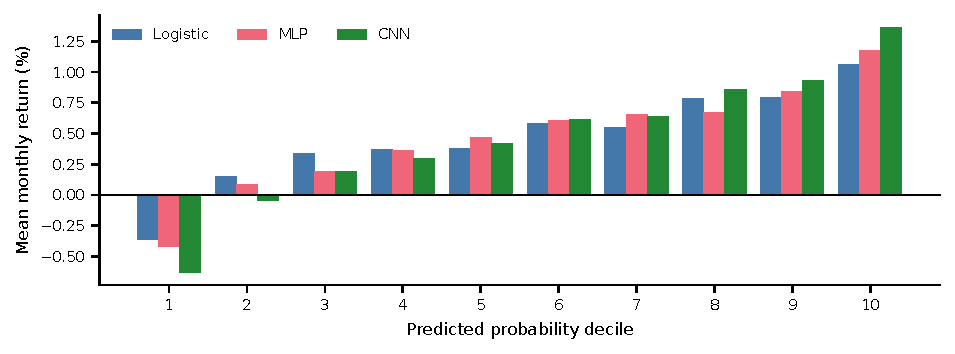
\includegraphics[width=0.82\linewidth]{figures/deciles.pdf}
\caption{Mean monthly return by predicted-probability decile, 2000--2019, probabilities averaged over seeds. Each date is sorted independently; decile 1 is the lowest predicted probability.}
\label{fig:deciles}
\end{figure}

Economic validity is where the story weakens. Splitting the sample, the monthly mean return of the CNN portfolio falls from 2.86\% in 2000--2004 to 1.55\% in 2005--2012 and 0.65\% in 2013--2019, with Sharpe ratios of 1.98, 2.61, and 1.24. The linear model's mean falls from 2.35\% to 1.23\% to 0.45\%, and the MLP's from 2.54\% to 1.37\% to 0.45\%. By the last block all three models deliver less than one percent per month gross, and at 20 basis points of one-way cost the seed-average net Sharpe ratios are 0.83, 0.78, and 0.87. The ranking information has not vanished, but the economic margin has compressed to the point where the result depends on cost assumptions.

\begin{figure}[t]
\centering
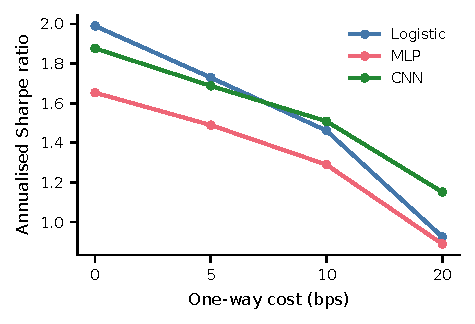
\includegraphics[width=0.55\linewidth]{figures/costs.pdf}
\caption{Annualised Sharpe ratio against one-way trading cost for the top-decile portfolio.}
\label{fig:costs}
\end{figure}

Turnover is high: $\tau\approx1.77$, so the portfolio replaces roughly 88\% of its gross book each month and a 10 basis point one-way cost removes about 35 basis points of monthly return. This is a structural property of re-ranking a large cross-section every month, and it means the gross Sharpe ratios in Table~\ref{tab:portfolio} are not attainable in practice.

\section{Question 3: a stable shape or a period-specific regularity?}

\textbf{Architecture ablations.} With a fixed 12{,}000-sample budget, four epochs, and three seeds, no architecture variant separates from the others: AUC ranges from 0.492 to 0.508 across two, three, and four blocks and narrow and wide filter stacks, and the decile Sharpe ratios are statistically indistinguishable from zero (Table~\ref{tab:ablation}). The budget is too small to train any of these models well, and the seed standard deviations of the full-data runs are of the same order as the differences between variants here, so this table is evidence about the protocol, not about architecture.

\begin{table}[t]
\centering
\small
\caption{Fixed-budget architecture ablation, 12{,}000 samples, 4 epochs, seeds 7/17/27 (mean $\pm$ standard deviation). Portfolio Sharpe annualised with 12 periods.}
\label{tab:ablation}
\begin{tabular}{lcccc}
\toprule
Configuration & AUC & AP & Decile Sharpe & 20\% Sharpe \\
\midrule
Logistic         & $0.504\pm0.004$ & $0.509\pm0.003$ & $0.215$ & $0.175$ \\
CNN 2 blocks     & $0.492\pm0.008$ & $0.500\pm0.004$ & $-0.213$ & $-0.014$ \\
CNN 3 blocks     & $0.493\pm0.009$ & $0.499\pm0.007$ & $0.161$ & $0.162$ \\
CNN 4 blocks     & $0.494\pm0.005$ & $0.501\pm0.003$ & $0.145$ & $0.052$ \\
CNN narrow       & $0.500\pm0.008$ & $0.504\pm0.006$ & $-0.054$ & $0.026$ \\
CNN wide         & $0.508\pm0.009$ & $0.513\pm0.009$ & $0.011$ & $0.117$ \\
\bottomrule
\end{tabular}
\end{table}

\textbf{Grad-CAM.} Figure~\ref{fig:gradcam} shows sixteen test examples, four from each confusion quadrant, chosen at high confidence and spread across 2000--2019. The maps concentrate on the right-hand columns, the most recent trading days, for true positives and false positives alike. False negatives drawn from the same period show flatter maps. The visual reading is that the network looks at recent price movement, with little evidence of a chart pattern spanning the whole window.

\begin{figure}[t]
\centering
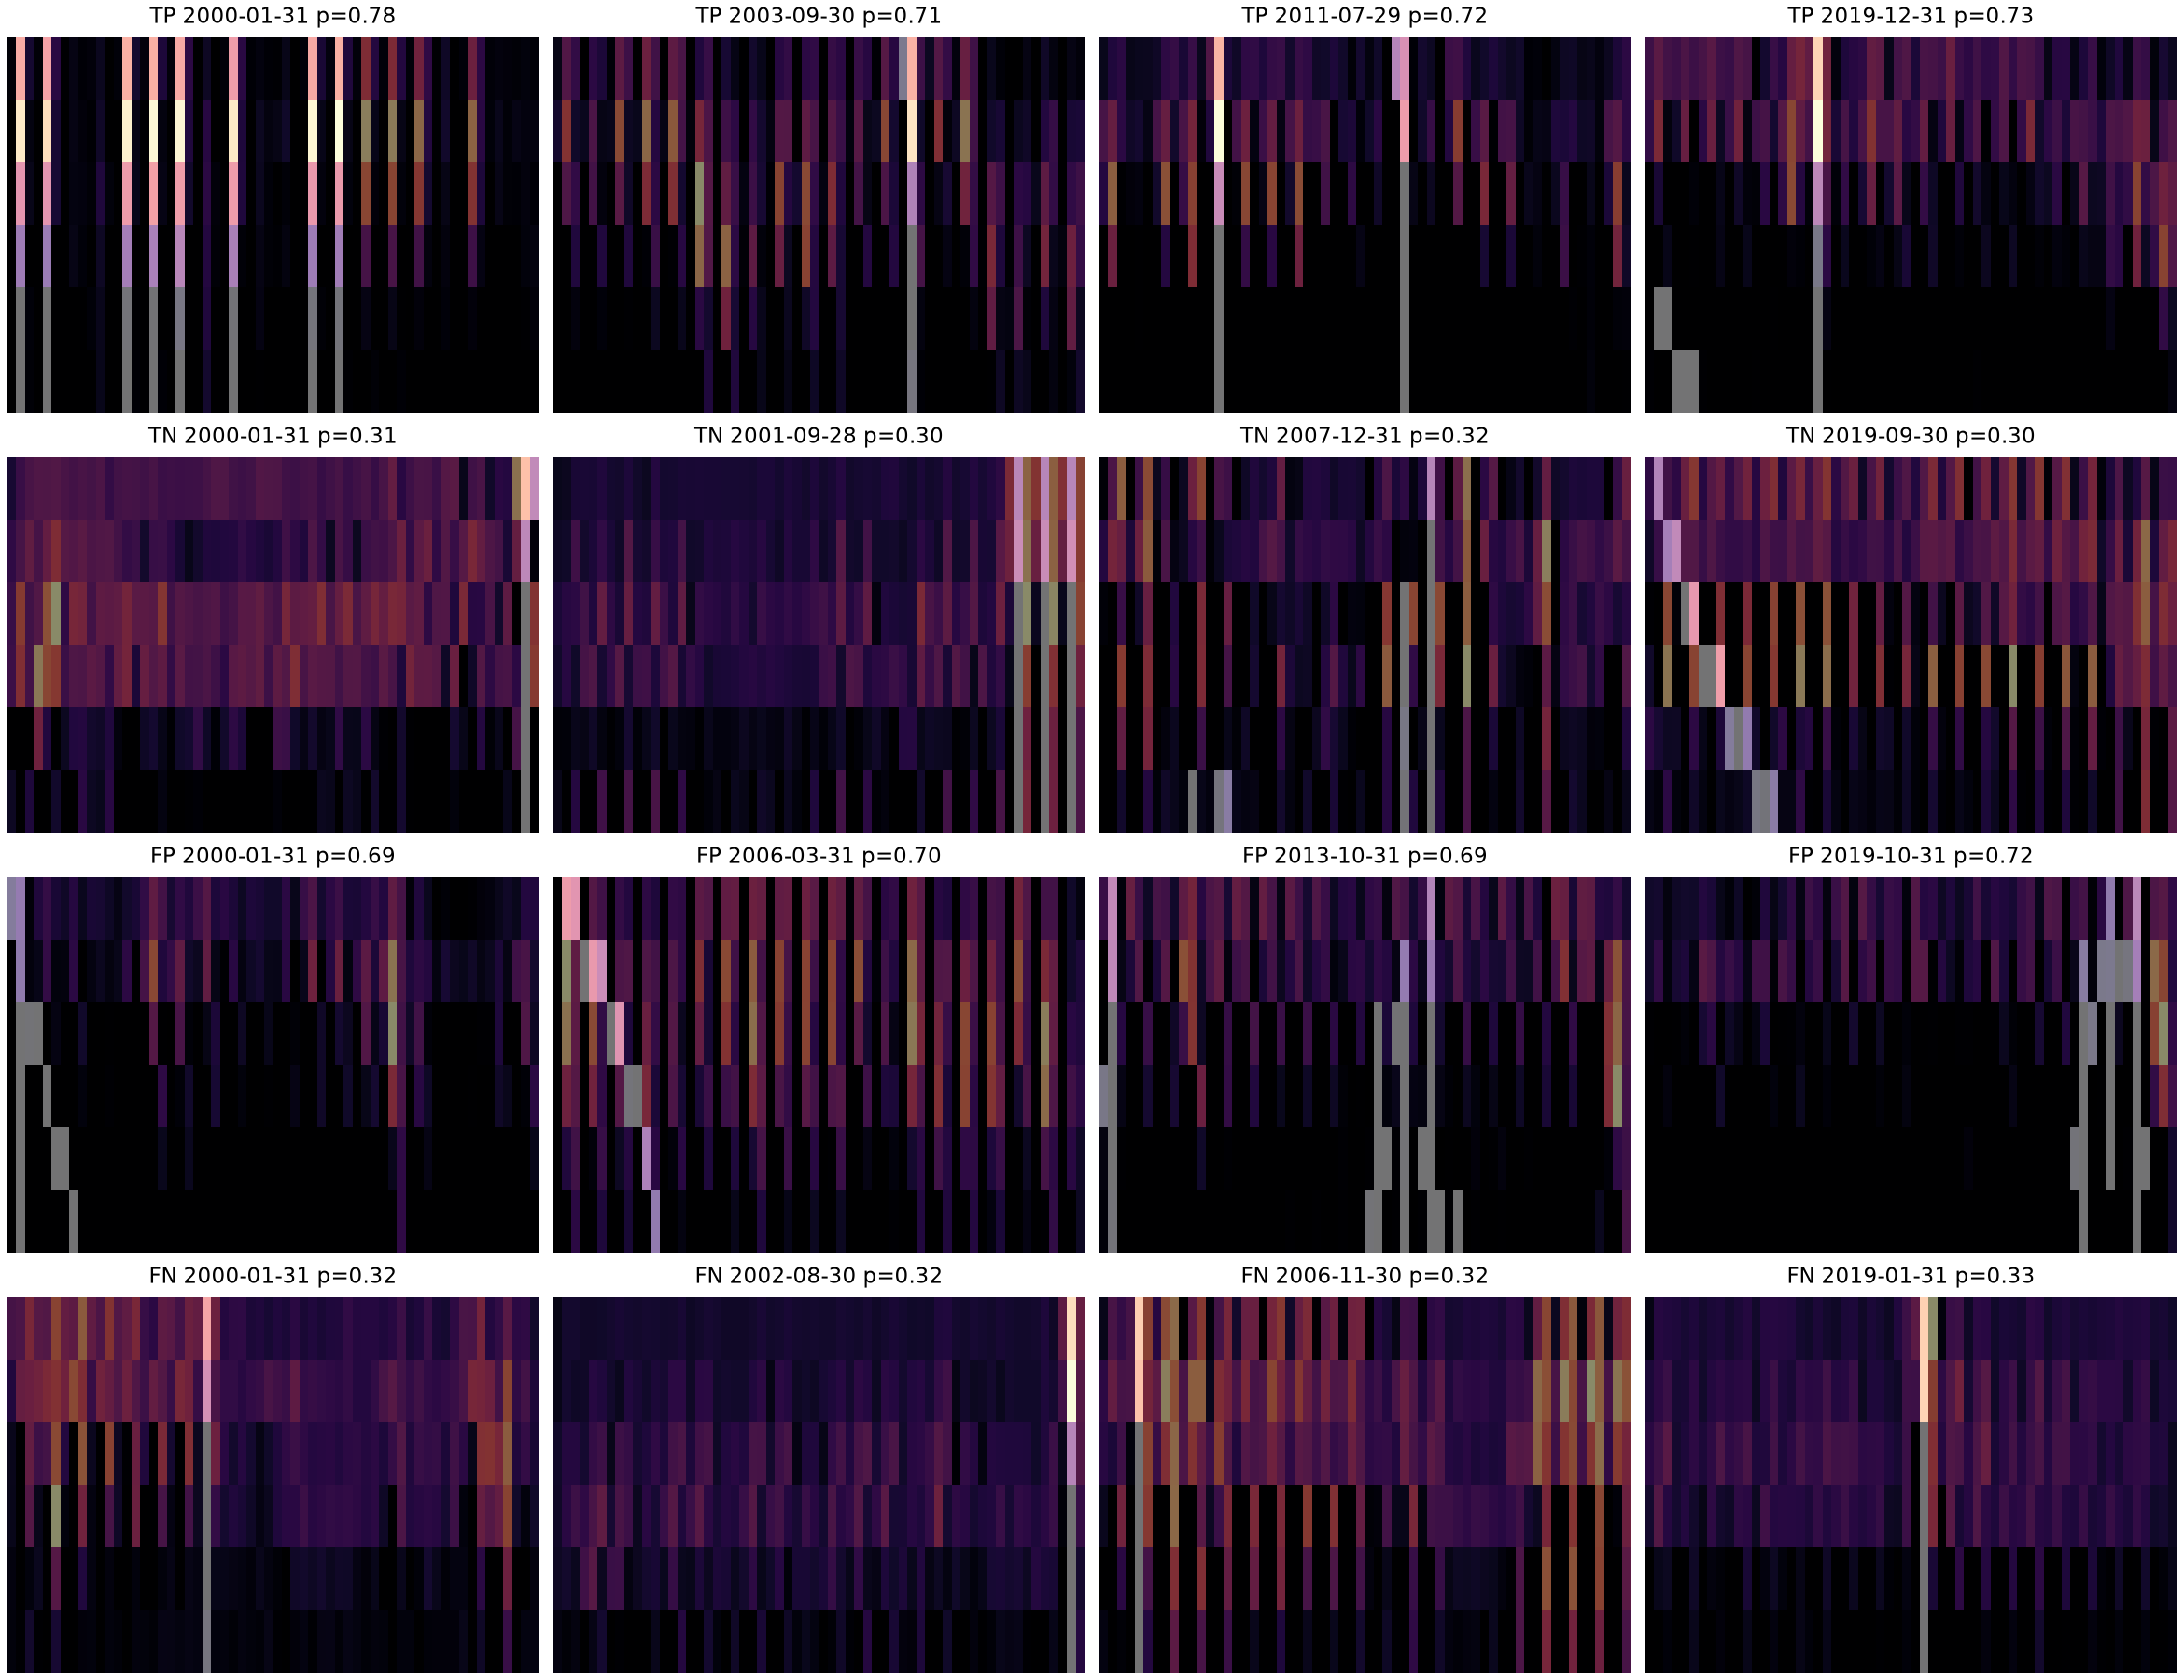
\includegraphics[width=\linewidth]{gradcam_full_16.png}
\caption{Grad-CAM for sixteen out-of-sample examples, four per confusion quadrant, from the checkpoint of the single hosted full-data run. Titles give the true label, date, and predicted probability. Warm colours mark high attribution.}
\label{fig:gradcam}
\end{figure}

\textbf{Occlusion.} Visual inspection cannot establish that the highlighted region is what the prediction depends on, so we remove it. On 200 high-confidence true positives we mask three columns of the input at a time and record the drop in predicted probability. Masking the three columns with the highest mean Grad-CAM attribution lowers the probability by 0.039 on average ($t=11.3$); masking three random columns lowers it by 0.010 ($t=5.8$); masking the three most recent columns lowers it by 0.080 ($t=17.6$); masking the three oldest columns slightly raises it ($-0.008$). The ranking of the interventions is informative: Grad-CAM points at columns that matter, roughly four times as much as random columns, but the recency of the column matters more than the attribution. The network's decision is dominated by the last few days of the image.

This is the sharpest answer we can give to Q3. The CNN does not appear to rely on a stable multi-week shape that can be transported across periods. It relies on the most recent part of the window, which is where a short-horizon momentum signal would sit, and the economic value of that signal falls exactly when the later sample stops rewarding it. The time decay of AUC and of portfolio returns is the same phenomenon observed from two directions.

\section{Limitations}

The study covers one dataset and one asset class, and the course panel ends in 2019; nothing here speaks to post-2019 behaviour. The portfolio analysis charges proportional costs but ignores borrow constraints, bid--ask spread heterogeneity, and market impact, all of which are material at monthly turnover near 180\%. The 20-day holding period and monthly rebalancing produce non-overlapping returns by construction, which keeps the $t$-statistics honest, but the resulting 240 observations limit the power of the subperiod comparisons. We train the main comparison with three seeds, which quantifies run-to-run variation for the headline numbers: seed standard deviations are 0.0038 in AUC and 0.35 in Sharpe for the CNN, so differences of a few thousandths in AUC or a few tenths in Sharpe should not be read as reliable rankings of models. The architecture comparison uses a fixed 12{,}000-sample budget rather than the full sample. Finally, the paper's development window (1993--2000) and test window (2001--2019) differ from the course split, so we replicate the specification rather than the exact experiment.

\section{Reproducibility, AI use, and contributions}

Code, configuration, and the scripts that regenerate every table and figure are at \url{https://github.com/imsf04/54_CNN}. The Kaggle notebook reproduces training on the hosted data; the local scripts reproduce the portfolio, attribution, and ablation analyses from saved predictions. Seeds, split logic, and normalisation statistics are fixed in code and recorded in the output files.

AI assistants were used to organise the code, locate errors, and edit documentation. The data audit, the runs, and the interpretation were checked by the author on the local machine and on the remote GPU host; every number in this report is produced by a script in the repository.

\textbf{Contributions.} PENG You designed the replication, implemented the pipeline, ran the experiments, and wrote this report.

\begin{thebibliography}{9}
\bibitem{jkx} Jiang, Z., Kelly, B., and Xiu, D. (2023). (Re-)Imag(in)ing price trends. \emph{Journal of Finance}, 78(6), 3193--3249.
\bibitem{gradcam} Selvaraju, R. R., Cogswell, M., Das, A., Vedantam, R., Parikh, D., and Batra, D. (2017). Grad-CAM: Visual explanations from deep networks via gradient-based localization. \emph{ICCV}.
\end{thebibliography}

\end{document}
